\subsubsection{Rule Offload}
\label{mazu-offload}

\begin{figure}
\centering
  \centering
  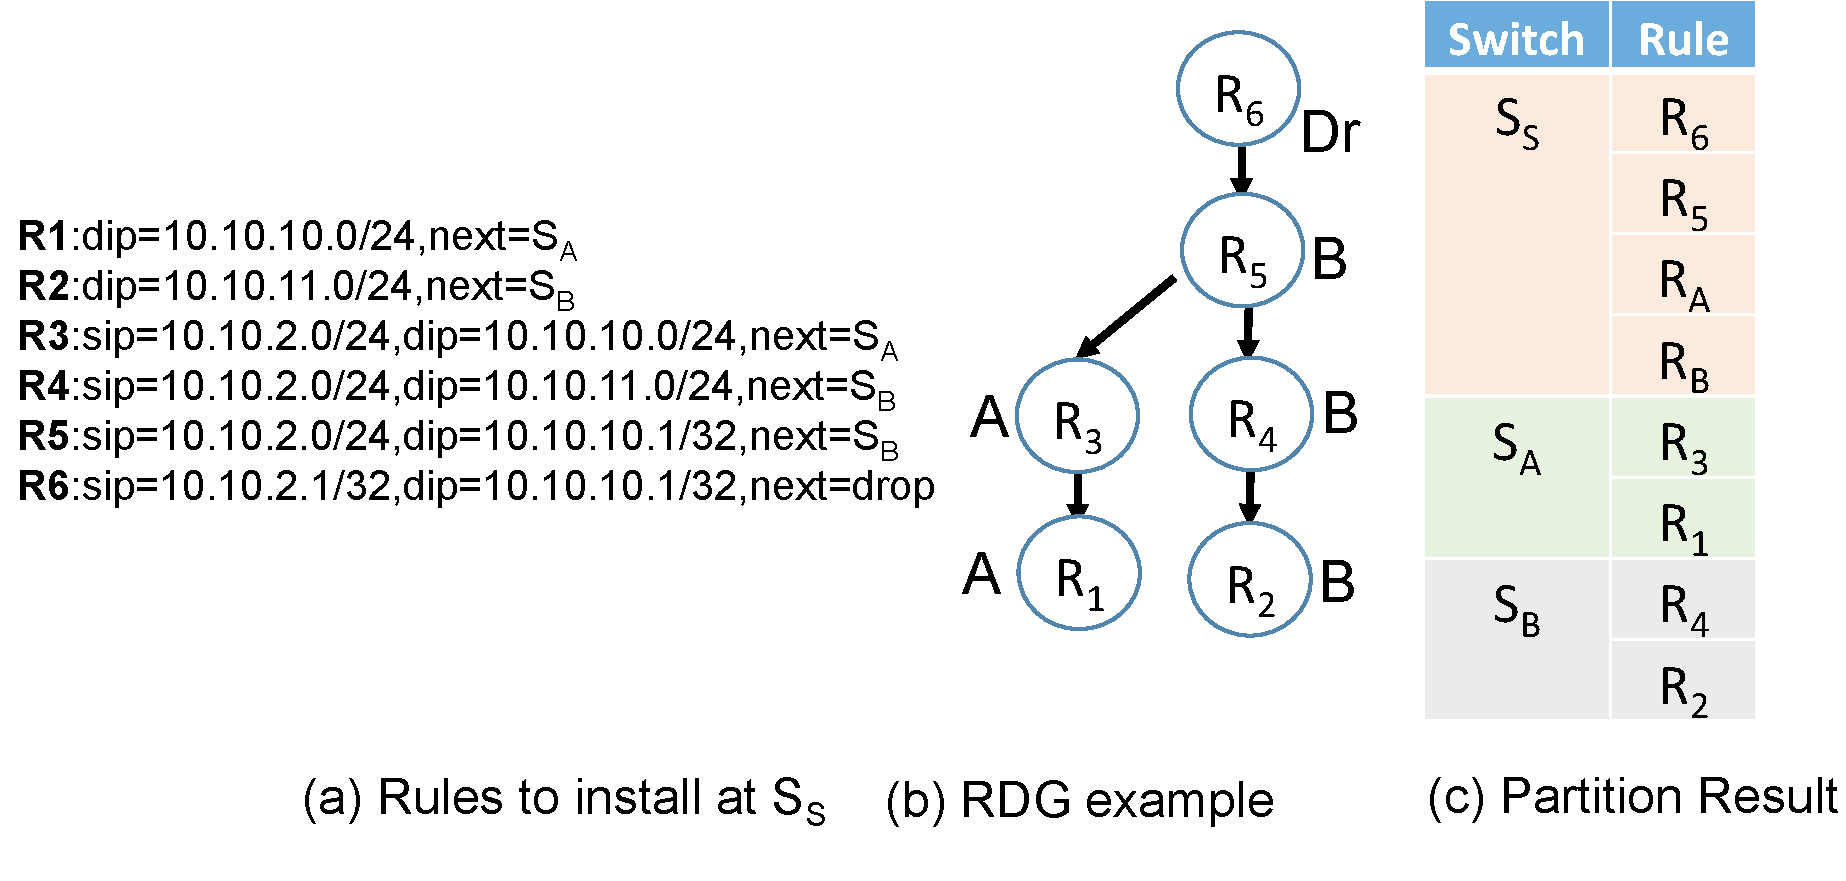
\includegraphics[width=0.55\textwidth]{figures/mazu/Rule-Offload2.pdf}
\caption{Rule offloading example}
\label{fig:rule-offload}
\end{figure}

When FE selects a path for a set of flows, the same number of rules are
installed/modified in every switch along the path. Thus, a path's update
latency is determined by the switch with the largest number of existing
low priority rules (assuming \BroadcomOne), or the largest number of pending
rule installations/modifications. For example, since switch $S_S$ in
\figref{fig:flow_eng} is part of all three paths to reach switch $S_D$, a
rule must be installed in $S_S$ for every new flow, regardless of whether the
flow traverses the path through $S_A$, $S_B$, or $S_C$.  Assuming
\BroadcomOne switches, it will take at least 0.3s to install rules for 100
flows of high priority $H$ in $S_S$---the same time required to install 20
rules in $S_A$ and longer than the $\approx$0.12s required to install 40
rules in both $S_B$ and $S_C$.

The goal of {\em rule offloading} (\RO) is to partition rules into subsets
that can be installed at downstream switches, with the appropriate {\em
default rules} installed at upstream switches. If the original number of
rules is $N$ and no partition (together with default rules) has more than $H$
rules, then, by updating the partitions in parallel, we can reduce rule
installation latency by a factor of $\frac{N}{H}$. 

Our algorithm consists of two phases. First, given a set of rules slated for
installation in a switch $S$ (called the {\em root} switch), we partition the
rules based on their next hop, taking into account any overlap between
rules. Second, we compute default rules for each partition; these rules are
installed in the root switch to direct packets to the next hop switch where
the original rules are actually installed.

\tightparagraph{Rule Partitioning Algorithm}
We represent the rules to be installed at a switch as a rule dependency graph
(RDG). In an RDG, a node denotes a rule, an edge represents a dependency
between two rules, and a node label indicates a rule's action (or next hop
switch). For example, \figref{fig:rule-offload}(b) depicts the RDG for the
six rules in \figref{fig:rule-offload}(a), which are slated for installation
in switch $S_S$ in the topology in \figref{fig:flow_eng}.  Note that when
rules send packets over a tunnel, we specify the next hop in the tunnel path,
not the tunnel destination, as the node label.

%\begin{algorithm}
\footnotesize
\DontPrintSemicolon
% \KwData{$G$: RDG with nodes annotated with next hop label, 
%	$H$: a bound of rule count for core switches,
%	$H_{core}$: the maximum number of rules any edge switch 
%           can offload to a core switch}
% \KwResult{$P$: partition set for next hops, initially empty}
%  \tcc{traverse reverse edges}
  %$N$ = min($H$, $H\_core$)\;
%  $G'$ = reverse($G$)\; 
    \SetKw{KwIn}{in}
    \SetKw{KwOr}{or}
    \SetKw{KwAnd}{and}
    \SetKwFunction{reverseBFS}{reverseBFS}
    \SetKwFunction{isLeaf}{isLeaf}
    \SetKwFunction{ruleCount}{ruleCount}
    \SetKwFunction{children}{children}
    \ForEach{$R$ \KwIn \reverseBFS{$G$}}{
%  \tcc{$R$ is the current node}
  $i$ = label($R$)\;
  \uIf{\isLeaf{$R$}}{
	 \uIf{\ruleCount{$P_i$} $> H_{down}$ \KwOr \ruleCount{$S_i$} $>H$} {
		$P_{root}$ += $R$\;
         }
         \Else{
             $P_i$ += $R$\;
	 }
   }
%   \tcc{$R$ depends on rules with more than one distinct label}
   \Else{
       \uIf{$\forall$ \children{$R$} $\in P_i$ \KwAnd
           \ruleCount{$P_i$} $> H_{down}$ \KwAnd \ruleCount{$S_i$} $>H$} {
             $P_i$ += $R$\;
           }
         \Else{
	    	$P_{root}$ += $R$\;
	 }
   }
 }
 \caption{Rule Partition}
 \label{alg:partition}
\end{algorithm}




The algorithm performs a reverse breadth-first
traversal of the RDG. If a node $R$ is a leaf node, then it is eligible to be
placed in partition $P_i$, where $i$ is $R$'s label (or next hop). A leaf
node $R$ is placed in $P_i$ if the current number of rules in $P_i$ is less
than $H_{down}$, otherwise $R$ is placed in $P_{root}$. $H_{down}$ controls 
the maximum number of rules we can offload to a switch downstream from the root switch. If a node $R$ is not
a leaf node, then it is only placed in partition $P_i$ if all of its children
are also in partition $P_i$, and the current number of rules in $P_i$ is less
than $H_{down}$. Otherwise, $R$ is placed in $P_{root}$.
The result is an allocation of rules $R \in RDG$ to the root switch ($S$) and
its next hops.
In the example (\figref{fig:rule-offload}), $R_1$ and $R_3$ are assigned to
partition $P_A$, $R_2$ and $R_4$ are assigned to $P_B$, and $R_5$ and $R_6$
are assigned to $P_{root}$. 
   

\tightparagraph{Computing Default Rules} 
Given the partitions for the next hop switches, we must compute a set of
default rules that {\em cover} the rules in each partition. These default
rules are added to $P_{root}$ to forward packets to the appropriate next hop
switch, where the rules in each partition (excluding $P_{root}$) are 
installed.
The main challenge is dealing with the fact that the intersection of default
rules may include rules from multiple partitions. 
Splitting the default rules into smaller rules can address this, but we must
be careful not to introduce too may default rules and undo the benefits of
RO.

Our heuristic from computing default rules is discussed below. Given the rules in a pair of partitions $P_i$ and
$P_j$, we create a {\em covering rectangle} for the rules in each partition,
denoted as $C_i$ and $C_j$. A covering rectangle is one whose source IP range
covers the entire source IP range specified in the rules in a partition;
likewise for destination IPs. This can easily be extended to higher
dimensions if rules are based on more than just source and destination IPs.

If the number of rules from either $P_i$ or $P_j$ in $C_i \cap C_j$ is below
a threshold $\Theta$, then all such rules are ``promoted'' to the root
partition $P_{root}$. We also create two default rules, one each for
$C_i$ and $C_j$, and install them in the root switch $S$.

If, however, the number of rules in $C_i \cap C_j$ exceeds $\Theta$, then we
further divide both $C_i$ and $C_j$ into two sub-rectangles, and we repeat
the process above for pairs of sub-rectangles, one from each partition.
We recursively repeat the process for a small number of steps. If at the
end of these steps, the combined number of default rules and rules in
$P_{root}$ is significant ($> \Omega$), then we merge $P_i$ and $P_j$ and
simply install all of their rules at the root switch $S$.

%\begin{algorithm}
\footnotesize
\SetKwFunction{defaultRule}{defaultRule}
\DontPrintSemicolon
% \KwData{rule partition set $P$}
% \KwResult{default rules at root and new partition set $P$}
  \SetKwFunction{proc}{checkOverlap}
    \SetKw{KwIn}{in}
    \SetKwFunction{ruleCount}{ruleCount}
%  $P'$ = $P$ - $P_{root}$\;
 \ForEach{distinct partition pair $(P_i, P_j)$ \KwIn $P$}{
  get covering rectangles $C_i$ and $C_j$ for $P_i$ and $P_j$\;
  \proc{$P$, $C_i$, $C_j$}\;
  }
  \SetKwProg{myproc}{Procedure}{}{}
  \myproc{\proc{$P$, $C_i$, $C_j$}} { 
  \uIf{\ruleCount{$C_i$ $\cap$ $C_j$} $\geq$ $\Theta$} {
   	divide $C_i$ and $C_j$ into two sub-rectangles each\;
	\ForEach{sub-rectangle pair ($C'_i$, $C'_j$)}{
		\proc{$P$, $C'_i$, $C'_j$}\;
	}
	
   }
   \Else{
        move $C_i$ $\cap$ $C_j$ to $P_{root}$\;
	$P_{root}$ += \defaultRule{$P_i$, $C_i$}\;
	$P_{root}$ += \defaultRule{$P_j$, $C_j$}\;
   }
  }
 \caption{Computing default rules}
 \label{alg:default_rule}
\end{algorithm}




We recursively apply RO to the switches in a set of paths, starting at the
ingress switch for the paths (e.g., $S_S$ in \figref{fig:flow_eng}),
followed by the second switch in each path, and so on.
The termination condition is that a set number of hops in each path are
explored. If at termination, the number of rules accommodated at every
switch, except the ingress switch, is $<H$, then we lower $H$ by a factor
$\gamma < 1$ and repeat again. If $H^*$ is the value of $H$ at the last of
such iterations, then we achieve a speedup of $\frac{N}{H^*}$ from installing
the offloaded rules in parallel. When running RO for an entire network, we
sort ingress switches in decreasing order of the number of rules to be 
installed and apply RO in this order. 
For simplicity, we have assumed that all the switches have the same latency
model; to accommodate switch diversity, we can assign different cost for the
rules offloaded to different core switches.


